\chapter{Summary of Research on Confidence}
	\label{cha:sum_confidence}
	
	This part of the thesis has discussed the machine intuition process of confidence: the act of suspicious processing of incoming data or uncertainty in the inferred information, and the communication of these doubts, in order to mitigate or completely stop the propagation of false information in automated processes.
	The communication and processing of confidence values is a larger concept, requiring the generation of confidence values at data sources, or the inference of confidence values at intermediate steps, as well as the use of confidence values in \ac{DL} model inference (Fig.~\ref{fig:gen_conf}).
	For all this, \acp{DNN} have to be extended to be able to digest and produce confidence values, which requires changes to the topology of the nets, as well as special techniques during training. 
	Furthermore, instead of the simple binary values we have investigated, the concept could be extended to a continuous range of confidence values, which requires the definition of what these fractional confidence values mean, and how to generate data that corresponds to them.

	\begin{figure}[ht]
		\centering
		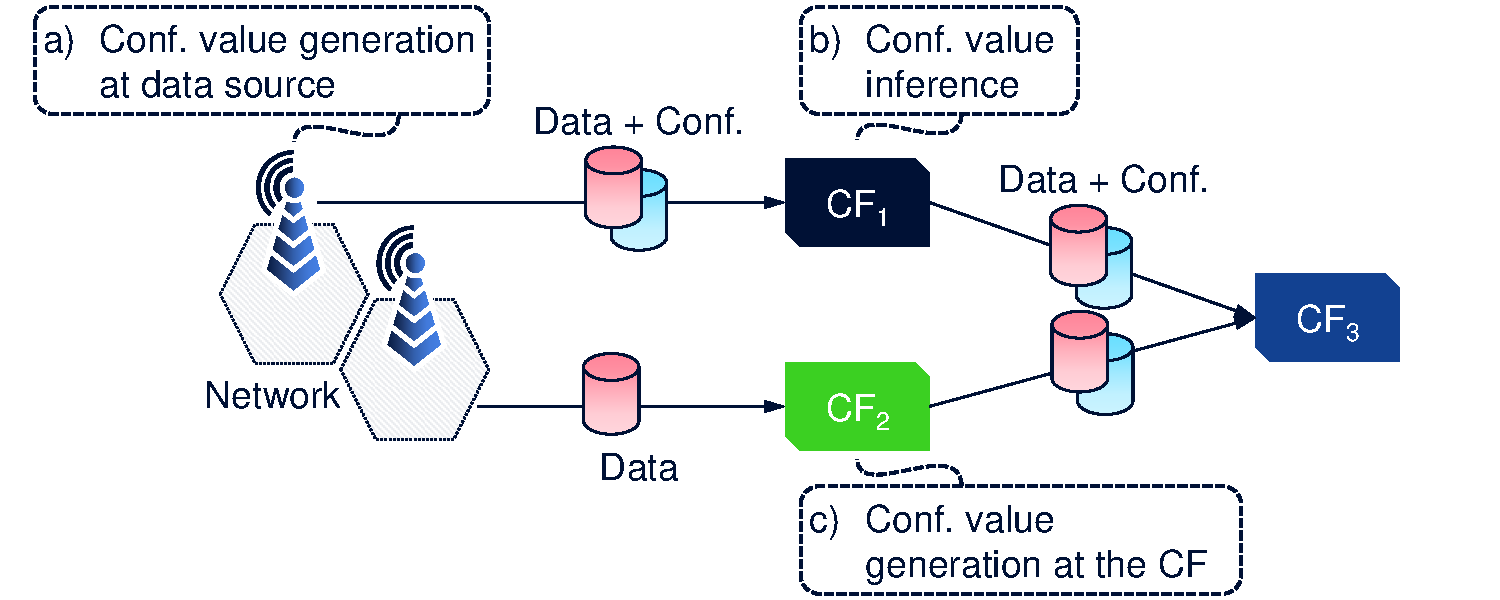
\includegraphics[width=\linewidth]{figures/13_sum_confidence/gen_conf/gen_conf.pdf}
		\caption[Confidence value sources in CAN]{Confidence value sources in CAN.}
		\label{fig:gen_conf}
	\end{figure}
	
	Our preliminary study focused on the use of confidence values in a simple scenario: the confidence values were attached to the inputs, either showing completely correct ($1.0$ confidence), or completely corrupted ($0.0$ confidence) data values.
	This scenario is called imputation, the replacement of missing values in datasets.
	To evaluate how well imputation works with \ac{DNN}-based \acp{FC} in a mobile network automation scenario, we considered two setups: 1) various \ac{DNN}-based and statistical imputation methods, which acted as a ``standalone'' preprocessing module for a later \ac{ML} task, and 2) an ``integrated'' imputation solution, where the imputation was fused into the \ac{DNN} undertaking the \ac{ML} task.
	Our results show that the integrated method outperforms standalone imputation, as well as requiring less computational resources and even  providing benefits for regular operation without missing data.
	I think these results are a promising sign for the overall confidence value concept.
	Naturally, I don't consider the research on this topic concluded, and there are plans to continue development towards a full machine-confidence-enabled \ac{CAN}, however, it is possible to draw some conclusions even with this limited research.
	
	\section{Assessment of Feasibility (A4.1)}
	
		As shown previously, the utilization of confidence values in \acp{DNN} is possible.
		Neural nets model correlation between features or patterns in time, and if redundant information is present, can use these connections in the data to restore information and thus, keep their inference precision up even in case some of the inputs are corrupted.
		The question is how much redundant information there is typically in mobile network data.
		While this is of course entirely dependent on the specific use case, in my experience redundant information is quite abundant in mobile networks data, either in \acp{KPI} that relate to the same underlying condition (radio quality, overall demand in the cell), or entities which interact/interfere with each other, thus information about other entities is represented in their logged data.
		
		The larger confidence value concept would require \acp{DNN} to generate confidence values accompanying their output.
		This is a much more complicated task than utilizing confidence values on the input, and it is unclear whether the output capability depends on available confidence values on the input.
		Fortunately, the topic of explainable \ac{AI} is an active field of research nowadays, which, among others, includes techniques aimed at measuring the confidence of \ac{DNN} outputs.
		These techniques could be utilized to produce confidence values, or they could be helpful in developing a \ac{DNN} which outputs confidence values itself.
		I think inferring confidence values is feasible, but we will have to research this topic further to be able to say for sure. 
		
	\section{Assessment of Practicality (A4.2)}
	
		As we have seen, the processing overhead of confidence values might be negligible, if the generation can also be integrated into the \acp{DNN} similarly to the utilization.
		However, the communication of confidence values will always entail a large amount of added information: in the simplest and worst case, every data value is accompanied by a confidence value, doubling the communication load for the \acp{CF}.
		Selective confidence values could lighten this load, by either only supporting confidence values to some features in the dataset, or only for larger data-elements, such as having a single confidence values for a complete observation, or multiple observations, such as a $10$ second interval in a time-series.
		However, these lower resolution confidence indication schemes might lose a lot of the benefits of the individual confidence values we experimented with.
		Thus, it is quite probable that only critical \acp{CF} will use machine confidence, while other, less important functionality will be kept less robust for the sake of conserving network resources. 
		
		Fallback systems might require the careful tuning of the parameters which govern when the system should fall back, or alert the operators to malfunction.
		Otherwise, training for the generation of confidence values might also require fine-tuned parameters.
		However, apart from these possibilities, it seems to me that machine confidence is quite user-friendly and does not necessitate much parameter tuning.
		
	\section{Assessment of Applicability (A4.3)}
	
		Increased robustness is desired in every aspect of the mobile network, thus, machine confidence is widely applicable to almost all functionality in network automation.
		Even in use cases where \acp{DNN} are guaranteed to not process corrupted information, the output of confidence values could still be beneficial: for example, in a predictive handover system, confidence values below a threshold could suppress the triggering of handovers, thus reducing the number of too early or ping-pong handovers.
		Confidence values are also an excellent way of gaining insight into the inner-logic of \ac{DL} models -- the focus of explainable \ac{AI} -- which is a hot topic of research nowadays.
		Generally, confidence values can be seen as \ac{DL} models capable of showing doubt: a very human trait, which could go a long way in building trust towards \ac{DL} in the users.
	